\documentclass[twocolumn, 12pt]{article}    % two-column because cheat sheets fit like that
\usepackage[utf8]{inputenc}
\usepackage{amsmath}    % allows math to happen
\usepackage{marvosym}
\usepackage{textcomp}
\usepackage{geometry}   % allows you to change the margins and headers/footers, and more
\usepackage{array}
\usepackage{wrapfig}
\usepackage{multirow} 
\usepackage{graphicx}   % allows for inclusion of graphics or several types, i think
\usepackage{float}      % SUPER  IMPORTANT. lets you tell LaTeX where to put your graphics, as opposed to where it feels
\usepackage{wrapfig}    % Lets text wrap around figures, more relevant for reports really
\usepackage{caption}
\usepackage{amssymb}    
\usepackage{ulem}       % allows strikethrough and some
\usepackage[table]{xcolor}  % enhances tables by allowing colors to happen. notably, as background/fill colors
\usepackage{bondgraph}  % allows bond graphs
\usepackage{caption}    % lots of control of captions and caption geometries
\usepackage{ragged2e}

\geometry{margin=.5in}      % this allows for a lot to fit on the page

\begin{document}
\footnotesize
\RaggedRight
\section*{Classical Controls}%%
\begin{equation*}
    t_{r1} \approx 2.2\tau \hspace{30pt} t_{r2} \approx\frac{1.8}{\tau} \hspace{30pt} t_{s1} \approx 4\tau \hspace{30pt} t_{s2} \approx\frac{4}{\zeta \omega_n}
\end{equation*}
\begin{equation*}
    t_P = \frac{\pi}{\omega_n\sqrt{1-\zeta^2}} \hspace{30pt} M_P = exp\left(\frac{-\pi\zeta}{\sqrt{1-\zeta^2}}  \right) \hspace{30pt} 
\end{equation*}
\begin{equation*}
    \%O.S. = M_P \times 100\% \hspace{30pt} \zeta = \frac{-ln(\%O.S./100)}{\sqrt{\pi^2 +ln^2(\%O.S. /100)}}
\end{equation*}
\begin{equation*}
    \delta \approx ln\left( \frac{y(t)}{y(t+\Delta t)} \right) \hspace{5pt} (\text{Log decrement}) \hspace{20pt} \zeta \approx \frac{\delta}{\sqrt{4\pi ^2 +\delta^2}} 
\end{equation*}
\begin{equation*}
    S_P^F = \lim_{\Delta P \to 0} \frac{\text{fractional change in function }F}{\text{fractional change in parameter }P}
\end{equation*}
\begin{equation*}
    S^F_P = \frac{P}{F}  \frac{\partial{F}}{\partial{P}} \hspace{30pt} 0 \equiv \text{not sensitive} \hspace{10pt} 1 \equiv \text{fully sensitive}
\end{equation*}

\subsection*{Op-Amps}%%
\begin{equation*}
    V_R(s) = RI(s) = Z_RI(s) \hspace{20pt} V_C(s) = \frac{1}{sC}I(s) = Z_c(s)I(s) 
\end{equation*}
\begin{equation*}
    V_L(s) = LsI(s) =Z_L(s)I(s)
\end{equation*}
\noindent
Take \textbf{either} path, not both
\begin{enumerate}
    \item In general: \(V_O = A(V^+-V^-)\)
    \item In negative feedback:
    \begin{enumerate}
        \item \(V^+ = V^-\)
        \item No current flows between "\(V^+\)" and "\(V^-\)"  \hspace{25pt} terminals
    \end{enumerate}
\end{enumerate}


\subsection*{Laplace Transform}
\begin{equation*}
    \mathcal{L}\{f(t)\} = F(s) = \int_{0^-}^\infty f(t)e^{-st}dt
\end{equation*}
\begin{equation*}
    \mathcal{L}\left\{\frac{d^nf(t)}{dt^n} \right\} = s^nF(s) - \sum^n_{i=1} s^{n-i} f^{n-1}(0)
\end{equation*}


\subsubsection*{Theorems}
\noindent
\begin{enumerate}
    \item \underline{Initial value}: \(\lim_{t\to 0^+} f(t) = \lim_{s\to \infty } sF(s)\) 
    \item \underline{Final value}: \textbf{iff} all roots of \(sF(s)\) are negative real, then \(f(\infty) = \lim_{t\to\infty} f(t) = \lim_{s\to0} sF(s)\)
\end{enumerate}

\subsection*{Standard Forms}
\begin{equation*}
    \frac{Y(s)}{R(s)} = K\frac{1/\tau}{s + 1/\tau} \hspace{30pt} \frac{Y(s)}{R(s)} = K\frac{\omega_n^2}{s^2+2\zeta\omega_ns+\omega_n^2}
\end{equation*}
\begin{equation*}
    D(s): s^2+2\zeta\omega_ns+\omega_n^2 =0 \hspace{10pt} \Longrightarrow \hspace{10pt} s_{1,2} = \zeta\omega_n \pm\jmath \omega_n\sqrt{1-\zeta^2}
\end{equation*}



\subsection*{Signal Flow Diagram}
\begin{enumerate}
    \item Label nodes (input/output signals, summing junctions)
    \item Assign each branch accordingly
    \item Label and define forward paths and loops
\end{enumerate}
\subsection*{Mason's Rule}
\begin{equation*}
    \frac{\text{output signal}}{\text{input signal}} = G_x(s) = \frac{1}{\Delta} \sum_i F_i\Delta_i
\end{equation*}
\begin{equation*}
    F_i = \text{path gain of } i^{th} \text{forward path from input to output} 
\end{equation*}
\begin{align*}
    \Delta = \text{s}&\text{ystem determinant}\\
            = 1 &- \sum (\text{all individual loop gains})\\
            & +\sum (\text{gain products of all possible combinations}\\
            & \text{\hspace{30pt}of \textbf{two} loops that do not touch})\\
            & -\sum (\text{gain products of all possible combinations}\\
            & \text{\hspace{30pt}of \textbf{three} loops that do not touch})\\
            & +\sum (\text{gain ... \textbf{four} loops ... do not touch})\\
            & -\sum (\text{gain ... \textbf{five} loops ... do not touch})\\
            & + .............. \hspace{10pt} \longrightarrow \hspace{10pt} \infty \text{ loops}\\
\end{align*}
\vspace{-40pt}
\begin{align*}
    \Delta_i &= i^{th}\text{ forward path determinant}\\
            &= \text{value of }\Delta \text{ for that part of the diagram}\\
            & \text{\hspace{10pt} that doe not touch the }i^{th} \text{ forward path }F_i
\end{align*}

\subsection*{Routh-Hurwitz Criterion}
\begin{enumerate}
\item \textbf{Fact 1}:
If there is at least one sign change in the coefficients of the \textbf{monic} polynomial, then there will be at least one pole \textbf{not} in the OLHP.\\
\item \textbf{Fact 2}:
If all coefficients of \textbf{monic} polynomial are positive, then we cannot say anything about the location of the poles.
\end{enumerate}
\noindent
if \(D(s) = s^n +a_1s^{n-1} + a_2s^{n-2} +... + a_n\), then the RH table will populate like this:
\begin{table}[H]
    \centering
    \begin{tabular}{c|cccc}
        \cline{2-5}
         \(s^n\) & \(1\)  & \(a_2\) &\(a_4\) & \dots  \\
         \(s^{n-1}\) &  \(a_1\) & \(a_3\) & \(a_5\) & \dots\\
         \cline{2-5}
         \(s^{n-2}\) & \(b_1\) & \(b_2\) & \(b_3\) & \dots\\
         \vdots & \(c_1\) & \(c_2\) & \(c_3\) & \dots\\
         \(s^0\) & \vdots & \vdots & \vdots & \(\ddots\)\\
    \end{tabular}
\end{table}
where the \(b_n\) and \(c_n\) coefficients are:\\
\begin{center}
\(
b_1 = -\frac{
\begin{array}{|cc|}
    1 & a_2 \\
    a_1 & a_3 
\end{array}} {a_1}
\) 
\hspace{10pt}
\(
b_2= -\frac{
\begin{array}{|cc|}
    1 & a_4 \\
    a_1 & a_5 
\end{array}} {a_1}
\) 
\hspace{10pt}
\(
b_3 = -\frac{
\begin{array}{|cc|}
    1 & a_6 \\
    a_1 & a_7 
\end{array}} {a_1}
\) \\
\vspace{10pt}
\(
c_1 = -\frac{
\begin{array}{|cc|}
    a_1 & a_3 \\
    b_1 & b_2 
\end{array}} {b_1}
\) 
\hspace{10pt}
\(
c_2= -\frac{
\begin{array}{|cc|}
    a_1 & a_5 \\
    b_1 & b_3 
\end{array}} {b_1}
\) 
\hspace{10pt}
\(
c_3 = -\frac{
\begin{array}{|cc|}
    a_1 & a_7 \\
    b_1 & b_5 
\end{array}} {b_1}
\) \\
\vspace{15pt}
\# sign changes in col. 1 = \# poles in ORHP
\end{center}
\subsubsection*{Special Cases}
\begin{enumerate}
    \item Replace any col. 1 zeroes with \(\epsilon\) (a teeny number)
    \item Replace any row of zeroes with \(d/ds\)(auxiliary polynomial) (generated from above row)
\end{enumerate}





\subsubsection*{Root Locus}
    RL techniques can be used for any arbitrary parameter \(\Gamma\), provided the char. eq. is of the form \(1+\Gamma \square =0\), where \(\square\) \hspace{5pt} is adapted to contain any term to make the form fit.
    \begin{equation*}
        1 +K \hat{G}(s) = 0 \hspace{50pt} |K\hat{G}(s)| = |-1|
    \end{equation*}
    
    \begin{equation*}
        \angle (K\hat{G}(s)) = 180^o + 360^o l, \hspace{30pt} l = 0 \pm 1, \pm 2, ...
    \end{equation*}
    
    \begin{align*}
        \angle \hat{G}(s) =& \Sigma \psi_i - \Sigma \phi_j\\
        =&+\Sigma(\text{angles from zeros to test point})\\ &- \Sigma(\text{angles from poles to test point})
    \end{align*}
    
    \begin{equation*}
        m \triangleq\text{number of zeroes} \hspace{30pt} n \triangleq \text{number of poles}
    \end{equation*}
    
    \begin{enumerate}
        \item Left of odd numbered poles/holes on real axis
        \item \(m\) poles go to \(m\) finite zeros, \(n\) poles go to \(m-n\) infinite zeros
            \begin{equation*}
                \lim_{K \to \infty} \hat{G}(s) = \lim_{K \to \infty} - \frac{1}{K} = 0
            \end{equation*}
        \item The poles move towards the zeros along asymptotes 
            \begin{equation*}
                \phi_h = \frac{180^o + 360^o (h-1)}{n-m} \hspace{30pt} h = 1,2,...,n-m
            \end{equation*}
        \item The location the asymptotes meet (center)
            \begin{equation*}
                \alpha = \frac{\Sigma Re(P_i) - \Sigma Re(z_j)}{n-m}    
            \end{equation*}
            
        \item Angles 
            \begin{equation*}
                q \triangleq \text{order of hole/pole,    } q>1 \Rightarrow \text{repeated holes/poles}
            \end{equation*}
            \begin{equation*}
                h \triangleq 1,2,3,...,q
            \end{equation*}
        \underline{Departures}
        \begin{equation*}
            q\phi_{dep} = (\Sigma \psi_i -\Sigma \phi_j) - 180^o - 360^o(h-1)
        \end{equation*}
        \(\psi_i=\) angles from zeroes to pole of interest\\
        \(\phi_j=\) angles poles to pole of interest\\
        
        \vspace{10pt}    
        \underline{Arrivals} 
        \begin{equation*}
            q\phi_{arr} = (\Sigma\phi_h -\Sigma\psi_k) + 180^o +360^o(h-1)
        \end{equation*}
        \(phi_h=\) angles from poles to zero of interest\\
        \(\psi_k=\) angles from zeroes to zero of interest\\
        
        \item The instability point is the \(K\) value that causes poles to land on the \(j\omega\)-axis. This is found by solving for the \(K\) that causes a row of zeroes to appear on a RH table. Then the auxiliary polynomial is solved for the \(\omega\) at that \(K\) value
        
        
        \item Breakaway/in points are found by manipulating the RL equation to solve for \(K(s)\). The \(s\) that satisfies \(\partial K(s)/ \partial s =0\) is the point
        
    \end{enumerate}
        
\subsubsection*{Bode Plots}

\subsubsection*{Ziegler-Nichols Tuning Methods}
\begin{enumerate}
    \item \underline{25\% Decay Approach} \\
        Assume an open-loop system has the following step-response. Finding \(L,R\) and selecting the following gains results in a Closed-Loop controller that reduces the oscillating overshoot to 25\% over the course of one period, with \(C(s)= K_P( 1 + 1/T_is + T_d s)\)
        \begin{figure}[h!]
            \centering
            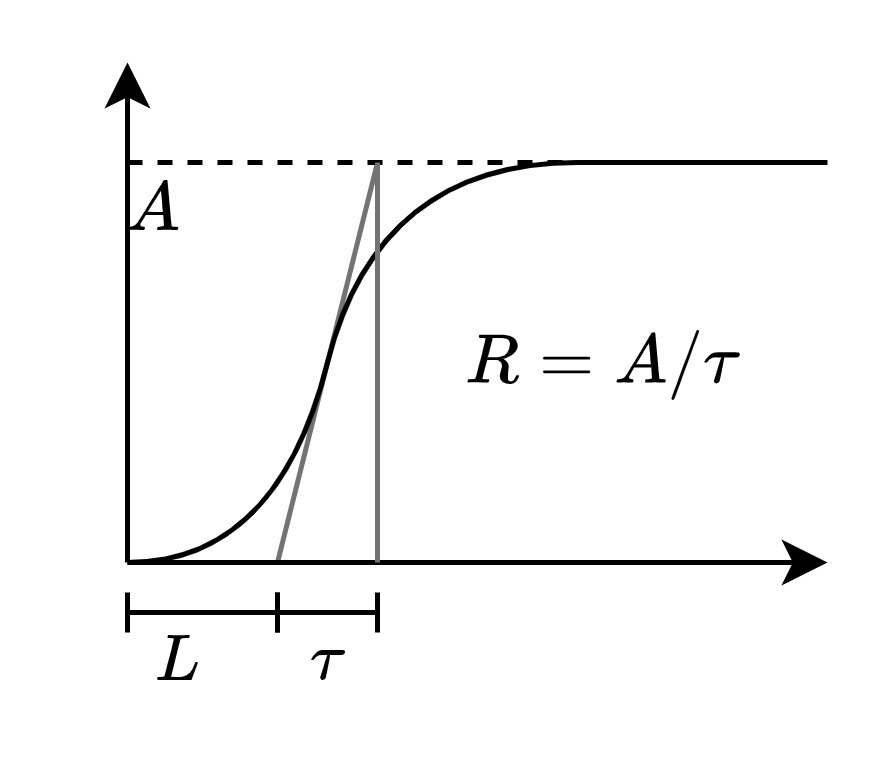
\includegraphics[width=0.3\textwidth]{ZNDecayApproach.jpg}
        \end{figure}
        
        \begin{table}[h!]
            \centering
            \begin{tabular}{|c|ccc|}
            \hline
                 &  Optimal Gains & &\\
                \hline
                P & \(K_P=1/RL\) & &\\
                PI & \(K_P=0.9/RL\) & \(T_i = L/0.3\)&\\
                PID & \(K_P = 1.2/RL\) & \(T_i = 2L\) & \(T_d=L/2\)\\
                \hline
            \end{tabular}
        \end{table}
        
    \item \underline{Ultimate Sensitivity Method}\\
        Starting with a closed-loop system, with reference = 0, increase \(K_P\) until marginal stability and measure \(Pu\) and \(K_P^*\). The optimal gains are given for \(C(s)= K_P( 1 + 1/T_is + T_d s)\)
            \begin{figure}[h!]
                \centering
                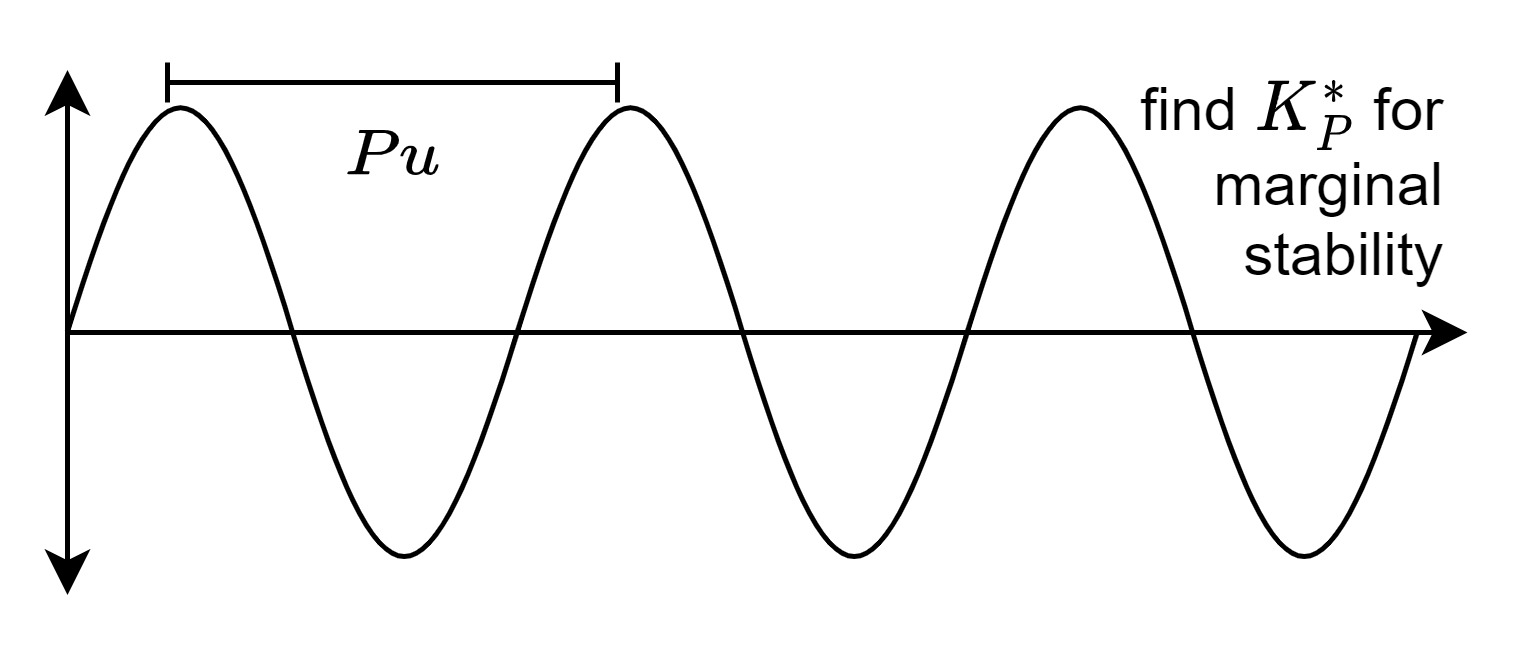
\includegraphics[width=0.40\textwidth]{ZNSensitivityApproach.jpg}
            \end{figure}
            
            \begin{table}[h!]
            \centering
            \begin{tabular}{|c|ccc|}
            \hline
                 &  Optimal Gains & &\\
                \hline
                P & \(K_P=K_P^*/2\) & &\\
                PI & \(K_P=0.45 K_P^*\) & \(T_i = Pu/1.2\)&\\
                PID & \(K_P = 0.6 K_P^*\) & \(T_i = Pu/2\) & \(T_d=Pu/8\)\\
                \hline
            \end{tabular}
        \end{table}
        
\end{enumerate}

\subsubsection*{Bode Plots}
Separate the TF into it's constitutive terms, and draw each term's Bode plot based upon it's type. The total Bode plot is the summation of each of the constitutive terms. System type \(n\) is \(dM(0)/d\omega = -20n\)
\begin{enumerate}
    \item \textbf{Type 1}: \hspace{30pt} \(K_0(j\omega)^n\), \hspace{15pt} \(n = 0, \pm 1, \pm2, \dots\)\\
    \underline{Magnitude}: Draw a line with slope = \(20n\) and intercept = \(20 log(K_0)\)\\
    \underline{Phase}: Draw a horizontal line at \(\phi = n(90^0\) 

    \item \textbf{Type 2}: \hspace{30pt} \((j\omega \tau +1)^{\pm1} \) \hspace{15pt}  \(\omega_{BP} = 1/\tau\)\\
    
    \underline{Magnitude}: Below \(\omega_{BP}\), the magnitude is 1 (0 dB). Above \(\omega_{BP}\), behaves like type 1.\\
    \underline{Phase}:\\
        \begin{enumerate}
            \item for \(\omega \tau  << 1\), then \(\angle(j\omega \tau +1)^{\pm1}  =0^o\) 

            \item for \(\omega \tau  >> 1\), then \(\angle(j\omega \tau +1)^{\pm1}  =90^o\) 
            
            \item for \(\omega \tau  \approx 1\), then \(\angle(j\omega \tau +1)^{\pm1}  \approx 45^o\) 
        \end{enumerate}
    
    \item \textbf{Type 3}: \hspace{2.5pt} \(\left[ \left( j\omega / \omega_n \right)^2 + 2 \zeta \left( j\omega/\omega_n \right) +1 \right] ^{\pm1}\) \hspace{2.5pt} \(\omega_{BP} = \omega_n\)\\
    The resonance at the peak is determined by \(\zeta\).
    
    \underline{Magnitude}: Same as type 2, but with slope \(\pm40\)\\
    \underline{Phase}: S-curves from 0 to \(\pm180^o\) crossing \(\omega_n\) at \(\pm90^o\)\\
\end{enumerate}

\textbf{Gain Margin}\\
Look at the phase plot of \(C(s)G(s)\) and find \(\omega_{GM}\) where phase \(= -180^o\). The distance between the plot and \(0dB\) at \(M(\omega_{GM})=GM\). \(GM>0\) is stable.

\textbf{Phase Margin}\\
Look at the magnitude plot of \(C(s)G(s)\) and find \(\omega_{PM}\) where magnitude \(=0dB\). The distance between the plot and \(-180^o\) at \(\phi(\omega_{PM})=PM\). \(PM>0\) is stable.\\

\begin{equation*}
    \text{if  } T(s) = \frac{\omega_n^2}{s^2+2\zeta\omega_ns + \omega_n^2} 
\end{equation*}
\begin{equation*}
    \text{then  } PM = tan^{-1} \left( \frac{2\zeta}{[(1+\zeta^4)^{1/2} - 2\zeta^2]^{1/2}} \right)
\end{equation*}

\begin{equation*}
    \text{if } 0\leq PM \leq 60 \text{  then  } PM=100\zeta
\end{equation*}


   
\subsubsection*{To Unity}
\begin{figure}[h!]
    \centering
    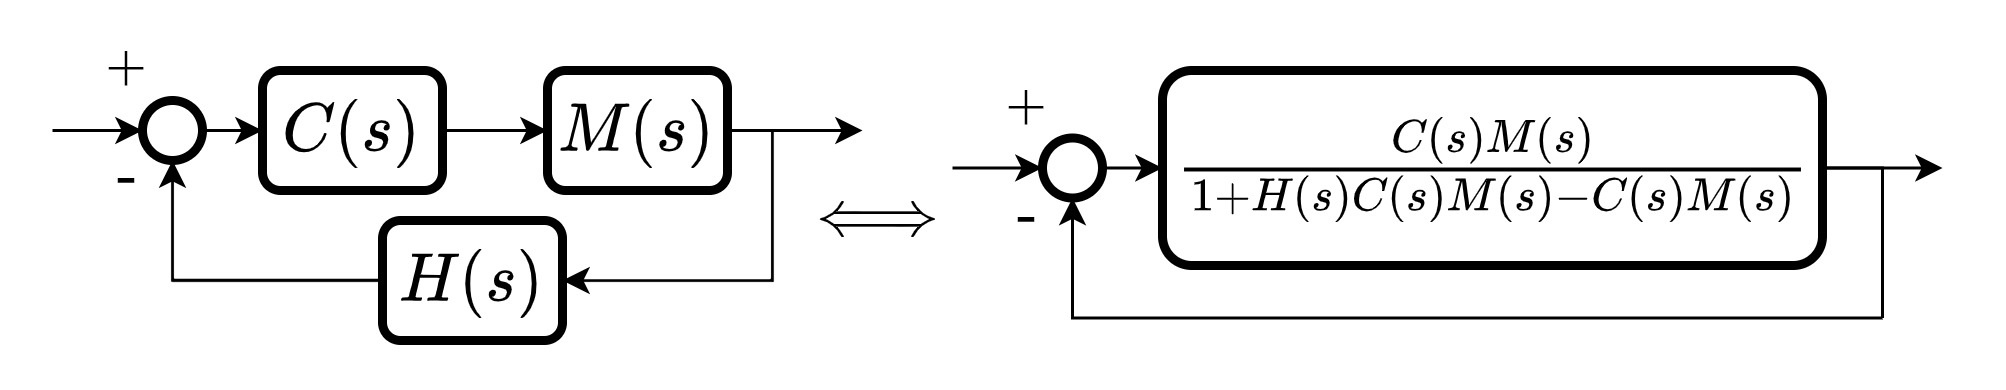
\includegraphics[width=0.45\textwidth]{SensorToUnity.jpg}
\end{figure}  
  
\subsection*{UNITY FEEDBACK ONLY}

\begin{equation*}
    \text{let } FP \triangleq \text{forward path} \hspace{30pt} \frac{E(s)}{R(s)} = \frac{1}{1+FP}
\end{equation*}

\begin{equation*}
    e_{ss} = \lim_{s\to0} sE(s) R(s) = \lim_{s\to0} s\left[ \frac{1}{1+FP} \right] R(s)
\end{equation*}


{\renewcommand{\arraystretch}{1.2}
\begin{table}[H]
    \centering
    \begin{tabular}{|c|c|c|c|}
        \hline
        Sys. Type & \(R(s)=\frac{A}{s}\)  & \(R(s) =\frac{A}{S^2}\) & \(R(s) = \frac{A}{s^3}\)\\
        \hline
        \(0\) & \(\frac{A}{1+K_P}\) & \(\infty\) & \(\infty\) \\
        
        \(1\) & \(0\) & \(\frac{A}{K_v}\) & \(\infty\)\\
        
        \(2\) & \(0\) &  \(0\) & \(\frac{A}{K_a}\) \\
        
        \(3\) & \(0\) & \(0\) & \(0\)\\
        \hline
    \end{tabular}
\end{table}}
\vspace{-20pt}
\begin{center}
    Match system type to input type to achieve \(e_{ss} =0\).
\end{center}
\begin{equation*}
    K_P = \lim_{s\to0}FP \hspace{30pt}  K_v = \lim_{s\to0} sFP \hspace{30pt} K_a=\lim_{s\to0}s^2FP
\end{equation*}



\subsection*{Analog Implementation}
\begin{figure}[h!]
    \centering
    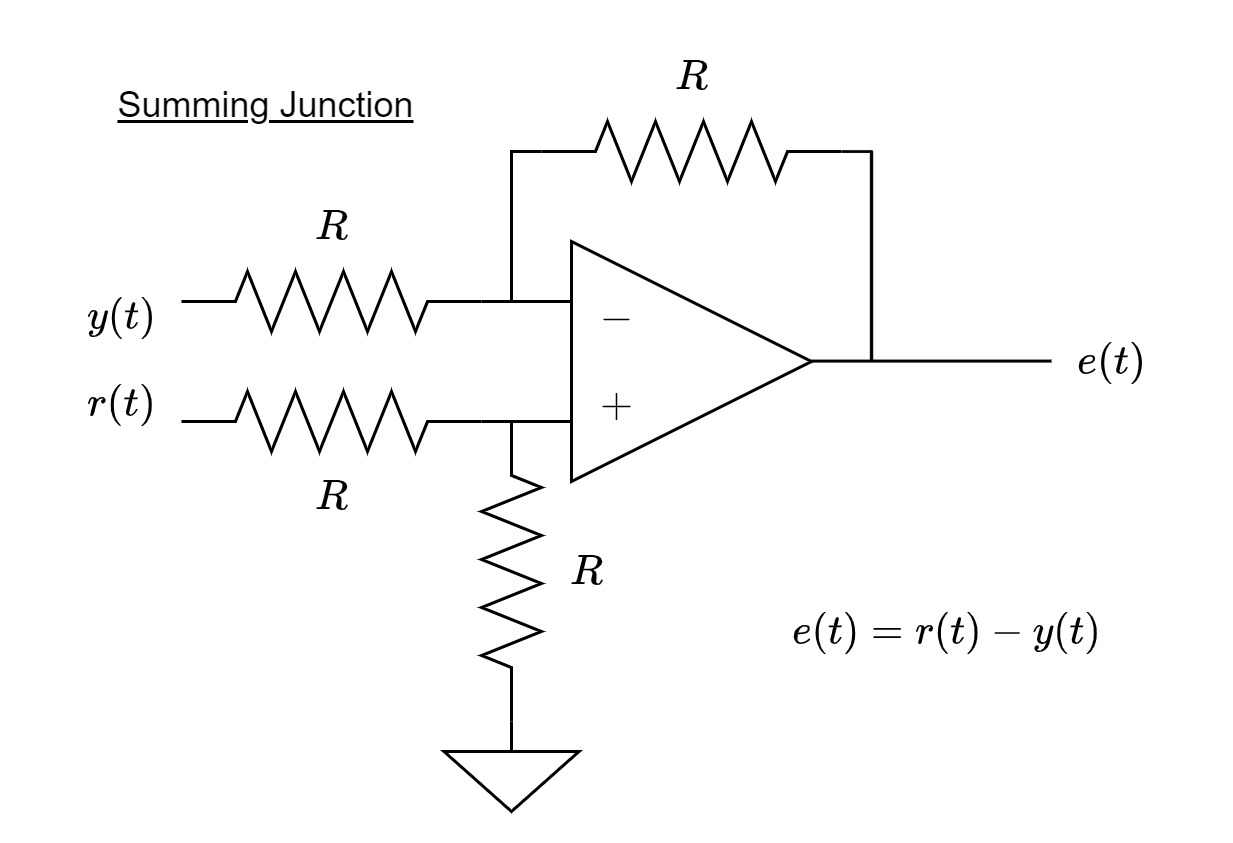
\includegraphics[width=0.33\textwidth]{AnalogController-SummingJunction.jpg}
\end{figure}
\begin{figure}[h!]
    \centering
    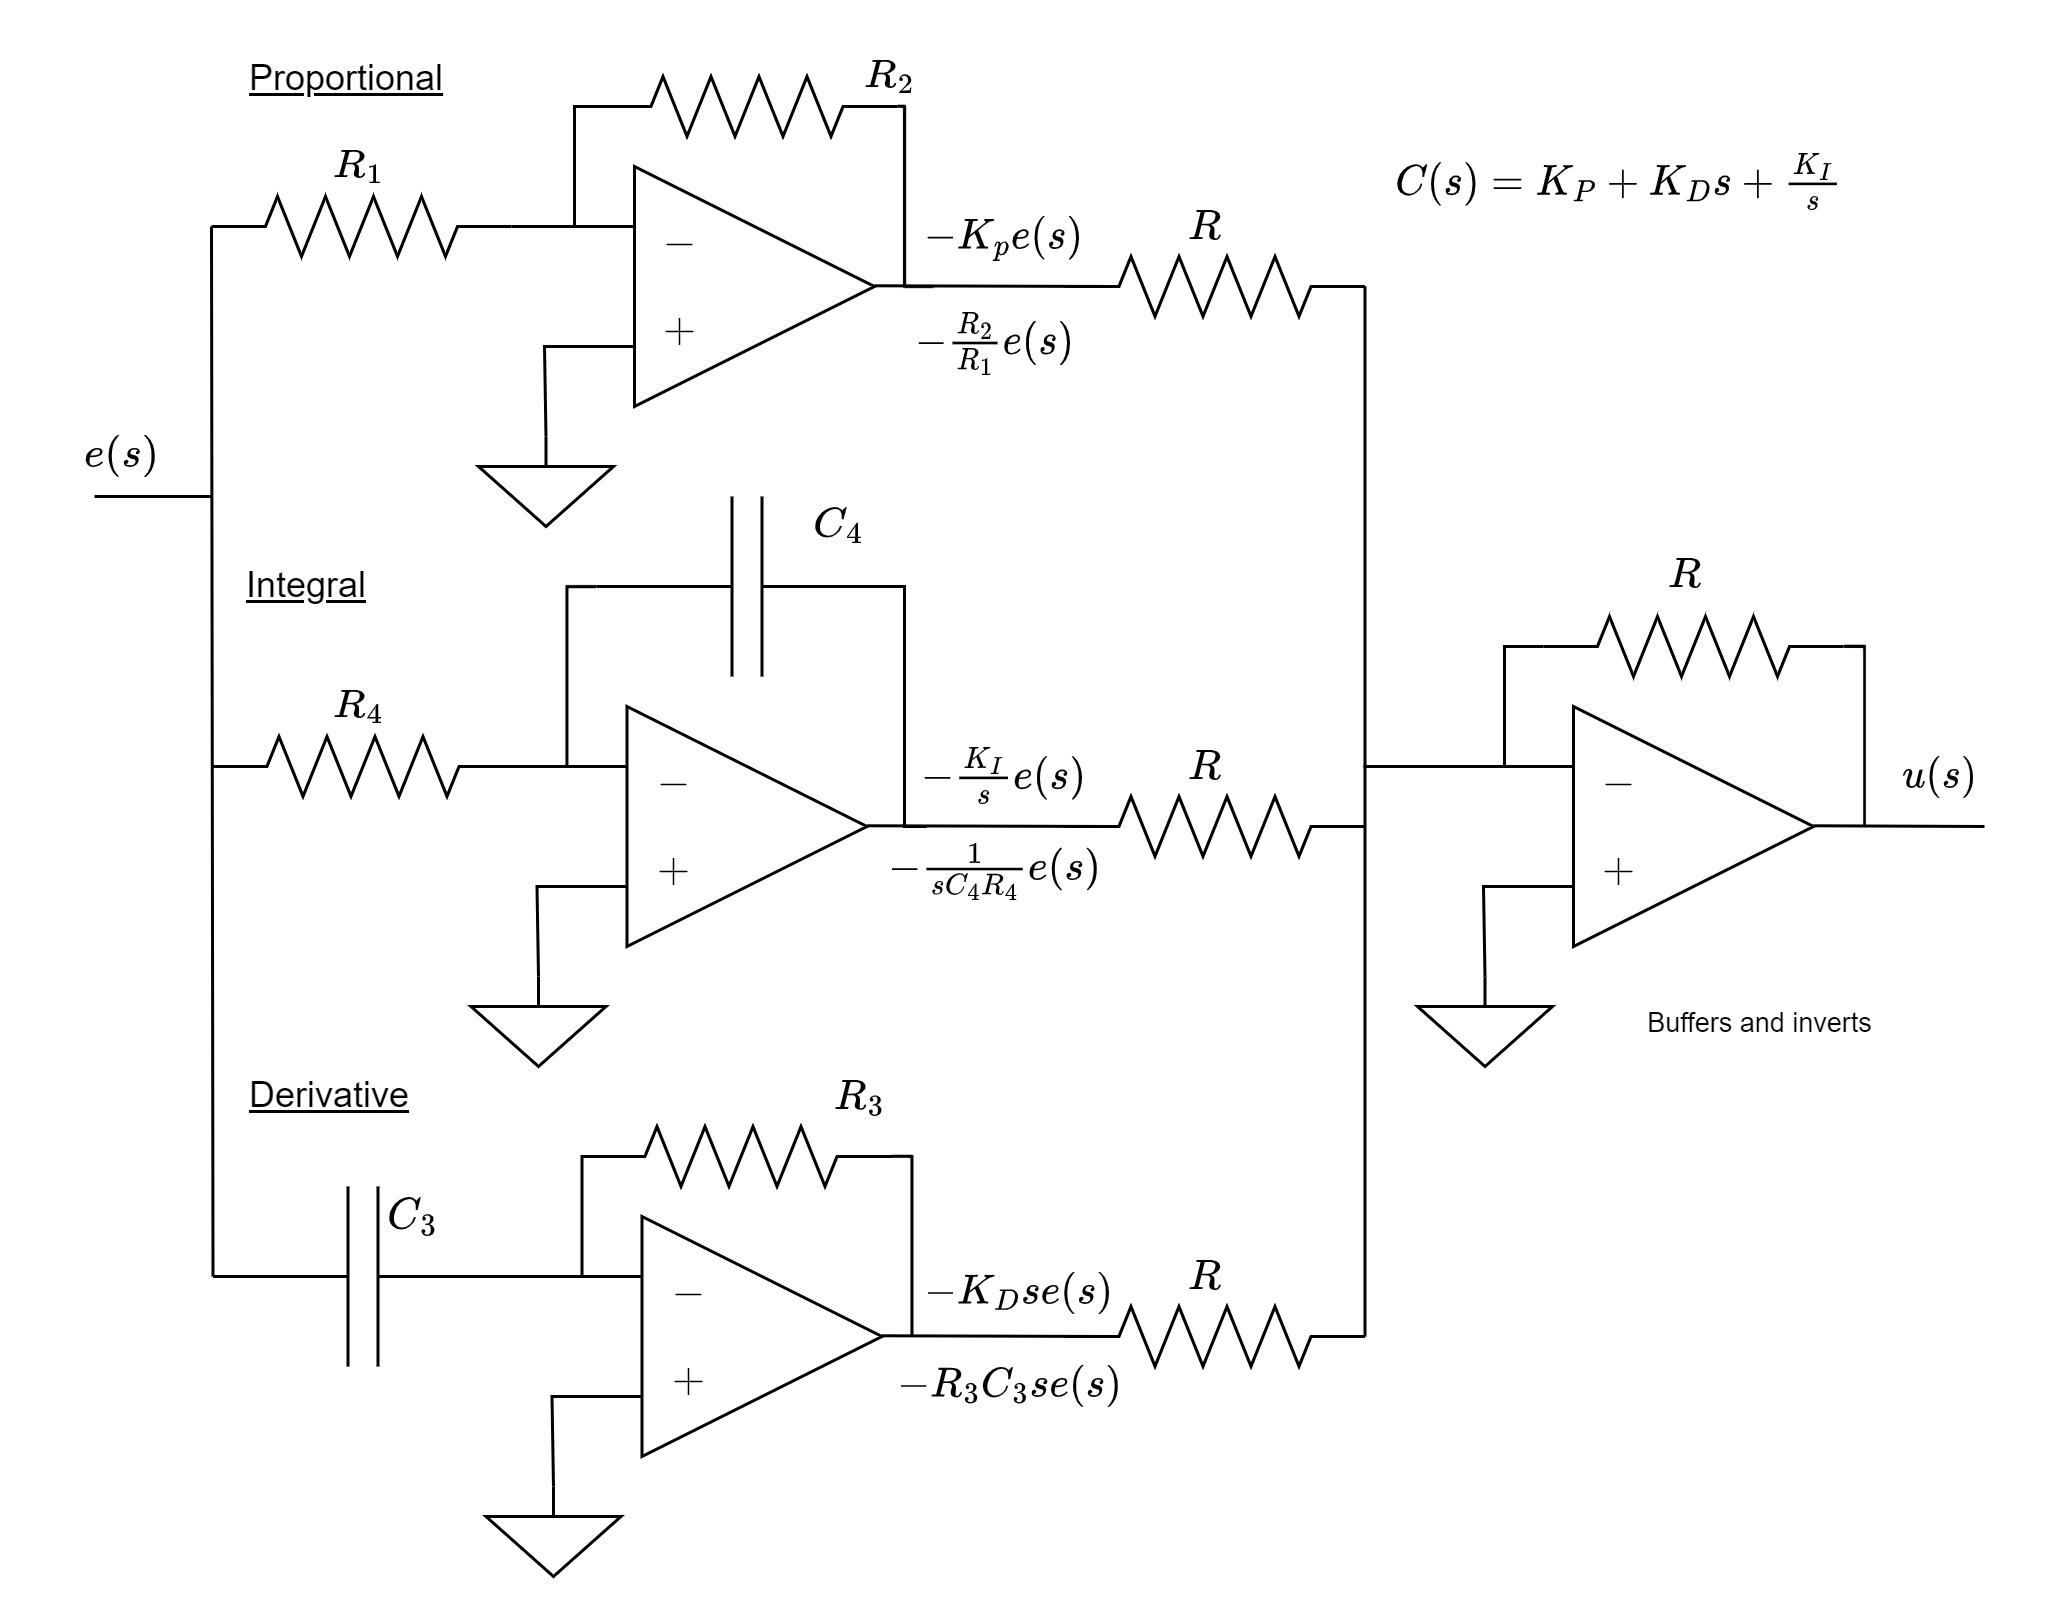
\includegraphics[width=0.45\textwidth]{AnalogController-PID_Controller.jpg}
\end{figure}
\begin{figure}[h!]
    \centering
    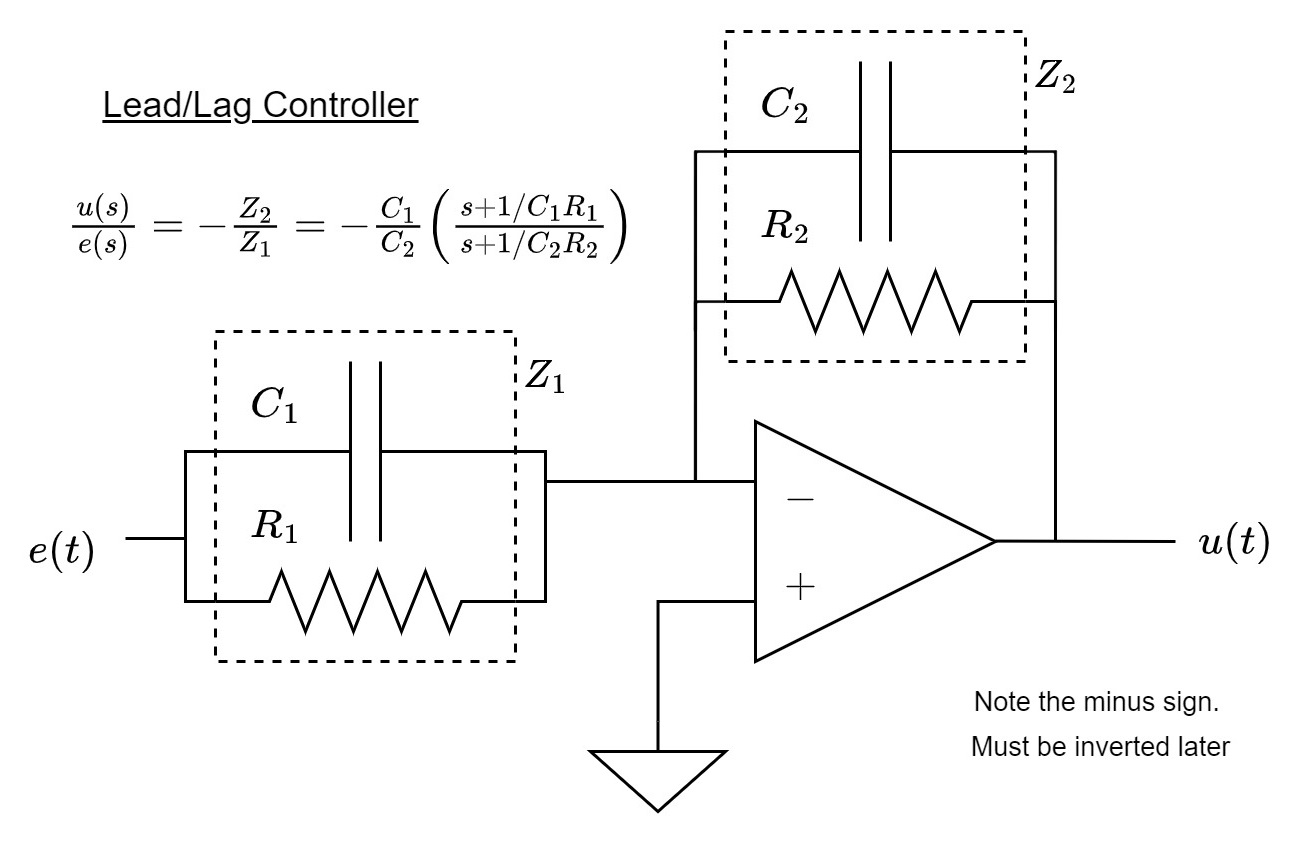
\includegraphics[width=0.45\textwidth]{AnalogController-Lead_LagController.jpg}
\end{figure}
\begin{figure}[h!]
    \centering
    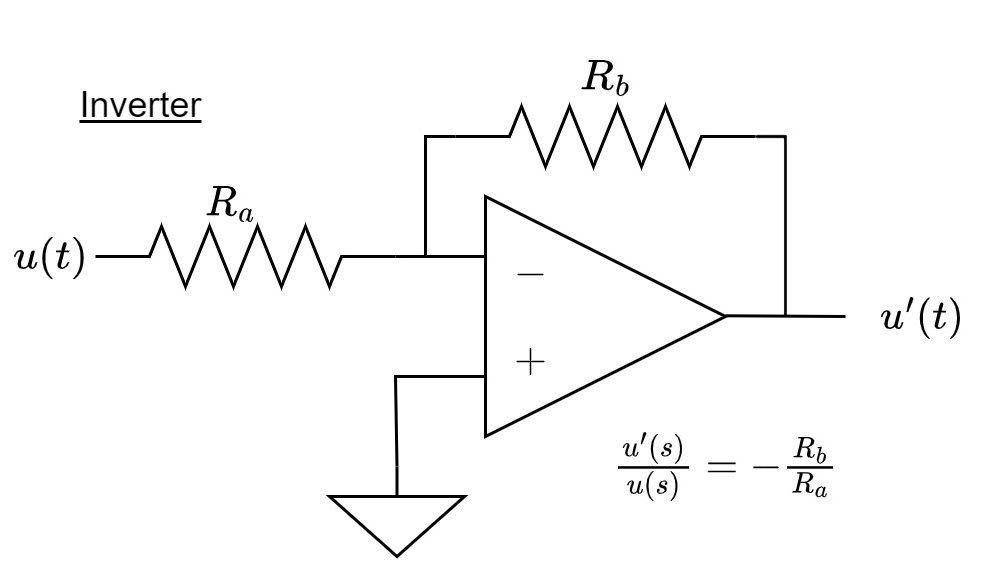
\includegraphics[width=0.33\textwidth]{AnalogController-Inverter.jpg}
\end{figure}


\end{document}